\documentclass[11pt,preprint]{elsarticle}

\usepackage{lmodern}
%%%% My spacing
\usepackage{setspace}
\setstretch{1.2}
\DeclareMathSizes{12}{14}{10}{10}

% Wrap around which gives all figures included the [H] command, or places it "here". This can be tedious to code in Rmarkdown.
\usepackage{float}
\let\origfigure\figure
\let\endorigfigure\endfigure
\renewenvironment{figure}[1][2] {
    \expandafter\origfigure\expandafter[H]
} {
    \endorigfigure
}

\let\origtable\table
\let\endorigtable\endtable
\renewenvironment{table}[1][2] {
    \expandafter\origtable\expandafter[H]
} {
    \endorigtable
}


\usepackage{ifxetex,ifluatex}
\usepackage{fixltx2e} % provides \textsubscript
\ifnum 0\ifxetex 1\fi\ifluatex 1\fi=0 % if pdftex
  \usepackage[T1]{fontenc}
  \usepackage[utf8]{inputenc}
\else % if luatex or xelatex
  \ifxetex
    \usepackage{mathspec}
    \usepackage{xltxtra,xunicode}
  \else
    \usepackage{fontspec}
  \fi
  \defaultfontfeatures{Mapping=tex-text,Scale=MatchLowercase}
  \newcommand{\euro}{€}
\fi

\usepackage{amssymb, amsmath, amsthm, amsfonts}

\def\bibsection{\section*{References}} %%% Make "References" appear before bibliography


\usepackage[numbers]{natbib}

\usepackage{longtable}
\usepackage[margin=2.3cm,bottom=2cm,top=2.5cm, includefoot]{geometry}
\usepackage{fancyhdr}
\usepackage[bottom, hang, flushmargin]{footmisc}
\usepackage{graphicx}
\numberwithin{equation}{section}
\numberwithin{figure}{section}
\numberwithin{table}{section}
\setlength{\parindent}{0cm}
\setlength{\parskip}{1.3ex plus 0.5ex minus 0.3ex}
\usepackage{textcomp}
\renewcommand{\headrulewidth}{0.2pt}
\renewcommand{\footrulewidth}{0.3pt}

\usepackage{array}
\newcolumntype{x}[1]{>{\centering\arraybackslash\hspace{0pt}}p{#1}}

%%%%  Remove the "preprint submitted to" part. Don't worry about this either, it just looks better without it:

 \def\tightlist{} % This allows for subbullets!

\usepackage{hyperref}
\hypersetup{breaklinks=true,
            bookmarks=true,
            colorlinks=true,
            citecolor=blue,
            urlcolor=blue,
            linkcolor=blue,
            pdfborder={0 0 0}}


% The following packages allow huxtable to work:
\usepackage{siunitx}
\usepackage{multirow}
\usepackage{hhline}
\usepackage{calc}
\usepackage{tabularx}
\usepackage{booktabs}
\usepackage{caption}


\newenvironment{columns}[1][]{}{}

\newenvironment{column}[1]{\begin{minipage}{#1}\ignorespaces}{%
\end{minipage}
\ifhmode\unskip\fi
\aftergroup\useignorespacesandallpars}

\def\useignorespacesandallpars#1\ignorespaces\fi{%
#1\fi\ignorespacesandallpars}

\makeatletter
\def\ignorespacesandallpars{%
  \@ifnextchar\par
    {\expandafter\ignorespacesandallpars\@gobble}%
    {}%
}
\makeatother


% definitions for citeproc citations
\NewDocumentCommand\citeproctext{}{}
\NewDocumentCommand\citeproc{mm}{%
\href{\#cite.\detokenize{#1}}{#2}\nocite{#1}}

\makeatletter
% allow citations to break across lines
\let\@cite@ofmt\@firstofone
% avoid brackets around text for \cite:
\def\@biblabel#1{}
\def\@cite#1#2{{#1\if@tempswa , #2\fi}}
\makeatother
\newlength{\cslhangindent}
\setlength{\cslhangindent}{1.5em}
\newlength{\csllabelwidth}
\setlength{\csllabelwidth}{3em}
\newenvironment{CSLReferences}[2] % #1 hanging-indent, #2 entry-spacing
{\begin{list}{}{%
	\setlength{\itemindent}{0pt}
	\setlength{\leftmargin}{0pt}
	\setlength{\parsep}{0pt}
	% turn on hanging indent if param 1 is 1
	\ifodd #1
	\setlength{\leftmargin}{\cslhangindent}
	\setlength{\itemindent}{-1\cslhangindent}
	\fi
	% set entry spacing
	\setlength{\itemsep}{#2\baselineskip}}}
{\end{list}}

\usepackage{calc}
\newcommand{\CSLBlock}[1]{\hfill\break\parbox[t]{\linewidth}{\strut\ignorespaces#1\strut}}
\newcommand{\CSLLeftMargin}[1]{\parbox[t]{\csllabelwidth}{\strut#1\strut}}
\newcommand{\CSLRightInline}[1]{\parbox[t]{\linewidth - \csllabelwidth}{\strut#1\strut}}
\newcommand{\CSLIndent}[1]{\hspace{\cslhangindent}#1}


\urlstyle{same}  % don't use monospace font for urls
\setlength{\parindent}{0pt}
\setlength{\parskip}{6pt plus 2pt minus 1pt}
\setlength{\emergencystretch}{3em}  % prevent overfull lines
\setcounter{secnumdepth}{5}

%%% Use protect on footnotes to avoid problems with footnotes in titles
\let\rmarkdownfootnote\footnote%
\def\footnote{\protect\rmarkdownfootnote}
\IfFileExists{upquote.sty}{\usepackage{upquote}}{}

%%% Include extra packages specified by user

%%% Hard setting column skips for reports - this ensures greater consistency and control over the length settings in the document.
%% page layout
%% paragraphs
\setlength{\baselineskip}{12pt plus 0pt minus 0pt}
\setlength{\parskip}{12pt plus 0pt minus 0pt}
\setlength{\parindent}{0pt plus 0pt minus 0pt}
%% floats
\setlength{\floatsep}{12pt plus 0 pt minus 0pt}
\setlength{\textfloatsep}{20pt plus 0pt minus 0pt}
\setlength{\intextsep}{14pt plus 0pt minus 0pt}
\setlength{\dbltextfloatsep}{20pt plus 0pt minus 0pt}
\setlength{\dblfloatsep}{14pt plus 0pt minus 0pt}
%% maths
\setlength{\abovedisplayskip}{12pt plus 0pt minus 0pt}
\setlength{\belowdisplayskip}{12pt plus 0pt minus 0pt}
%% lists
\setlength{\topsep}{10pt plus 0pt minus 0pt}
\setlength{\partopsep}{3pt plus 0pt minus 0pt}
\setlength{\itemsep}{5pt plus 0pt minus 0pt}
\setlength{\labelsep}{8mm plus 0mm minus 0mm}
\setlength{\parsep}{\the\parskip}
\setlength{\listparindent}{\the\parindent}
%% verbatim
\setlength{\fboxsep}{5pt plus 0pt minus 0pt}



\begin{document}



\begin{frontmatter}  %

\title{Local Coffee Report}

% Set to FALSE if wanting to remove title (for submission)












\vspace{1cm}





\vspace{0.5cm}

\end{frontmatter}

\setcounter{footnote}{0}



%________________________
% Header and Footers
%%%%%%%%%%%%%%%%%%%%%%%%%%%%%%%%%
\pagestyle{fancy}
\chead{}
\rhead{}
\lfoot{}
\rfoot{\footnotesize Page \thepage}
\lhead{}
%\rfoot{\footnotesize Page \thepage } % "e.g. Page 2"
\cfoot{}

%\setlength\headheight{30pt}
%%%%%%%%%%%%%%%%%%%%%%%%%%%%%%%%%
%________________________

\headsep 35pt % So that header does not go over title




\section{Loading data and cleaning}\label{loading-data-and-cleaning}

I first inspect the raw data to assess how and what to clean. The
dataset has 145 columns, with many containing a large amount of missing
values. The columns relevant to the current analysis, such as loan
status, grade, and home ownership are all relatively complete.

To clean the data, I select only the relevant columns. Furthermore, I
create a binary outcome variable for whether the loan status is fully
paid off or not. The summary statistics of the cleaned data indicate
outliers are present in the data. For instance, annual income has a
maximum of 9 500 000. Similarly, debt-to-income also has a hanful of
extreme outliers, with a handful of pre-cleaning observations with a dti
equal to 999. The cleaning drops the most extreme dti observations.

\begin{longtable}[]{@{}lrrrrr@{}}
\caption{Summary statistics}\tabularnewline
\toprule\noalign{}
variable & mean & median & sd & min & max \\
\midrule\noalign{}
\endfirsthead
\toprule\noalign{}
variable & mean & median & sd & min & max \\
\midrule\noalign{}
\endhead
\bottomrule\noalign{}
\endlastfoot
emp\_length & 6.1 & 6 & 3.6 & 1.0 & 10 \\
dti & 18.8 & 18 & 10.5 & 0.0 & 822 \\
annual\_inc & 78865.8 & 66000 & 80722.6 & 0.0 & 9550000 \\
int\_rate & 13.0 & 12 & 5.0 & 5.3 & 31 \\
default & 0.2 & 0 & 0.4 & 0.0 & 1 \\
\end{longtable}

\section{Default rates on short-term
loans}\label{default-rates-on-short-term-loans}

First, I filter to short-term loans, and then create a function which
calculates the default rate for any group. Among short term loans (36
months), the default rate falls as home ownership improves. Renters
default at 23.1\%, compared to 19.9\% for owners and 15.2\% for those
still paying a mortgage. This provides an indication that owning vs
renting matters. Although, the fact that mortgage holders default less
than owners is a less intuitive result.

\begin{longtable}[]{@{}lrr@{}}
\caption{Default rate by home ownership}\tabularnewline
\toprule\noalign{}
home\_ownership & n & default\_rate \\
\midrule\noalign{}
\endfirsthead
\toprule\noalign{}
home\_ownership & n & default\_rate \\
\midrule\noalign{}
\endhead
\bottomrule\noalign{}
\endlastfoot
MORTGAGE & 139189 & 15.2 \\
RENT & 120789 & 23.1 \\
OWN & 37406 & 19.9 \\
ANY & 63 & 20.6 \\
\end{longtable}

\begin{longtable}[]{@{}rrr@{}}
\caption{Default rate by employment length}\tabularnewline
\toprule\noalign{}
emp\_length & n & default\_rate \\
\midrule\noalign{}
\endfirsthead
\toprule\noalign{}
emp\_length & n & default\_rate \\
\midrule\noalign{}
\endhead
\bottomrule\noalign{}
\endlastfoot
5 & 18329 & 18.8 \\
10 & 96678 & 17.0 \\
3 & 24559 & 19.3 \\
4 & 17909 & 19.0 \\
1 & 44381 & 19.6 \\
8 & 12735 & 18.2 \\
NA & 21655 & 27.9 \\
6 & 12526 & 17.9 \\
9 & 10905 & 18.6 \\
2 & 27805 & 19.0 \\
7 & 9965 & 18.5 \\
\end{longtable}

\begin{figure}[H]

{\centering 
\includegraphics{22921893Question3_files/figure-latex/unnamed-chunk-4-1} 

}

\caption{Home ownership and default rates.}\label{fig:unnamed-chunk-4}
\end{figure}

Employment length does not appear to be a meaningful indicator of
default on short-term loans. Employees with 10+ years have a slightly
lower default rate, although the default rates between all employment
length groups is very similar. The one notable exception is the group
with a missing employment length, which defaults at 27.9\%. This is
possibly attributable to unemployed or self-employed individuals, who do
not report their employment length.

\begin{longtable}[]{@{}lrrr@{}}
\caption{Income of missing employment oberservations}\tabularnewline
\toprule\noalign{}
emp\_missing & n & mean\_income & median\_income \\
\midrule\noalign{}
\endfirsthead
\toprule\noalign{}
emp\_missing & n & mean\_income & median\_income \\
\midrule\noalign{}
\endhead
\bottomrule\noalign{}
\endlastfoot
FALSE & 275792 & 79248.64 & 65000 \\
TRUE & 21655 & 49109.66 & 42700 \\
\end{longtable}

\section{State differences in short-term loan
defaults}\label{state-differences-in-short-term-loan-defaults}

Now, I analyse differences in the defaults on short-term loans by state.
There is significant variability in the average default rate across
states. States such as Arkansas, Oklahoma, Louisiana, and Alabama have
the highest default rates with more than 20\%. The map plot confirms
that there are interstate differences in short-term loan defaults.
Specifically, Southern States have a higher propensity to default. The
states with the lowest propensity to default are more Northern, coastal
states, such as Oregon.

\begin{figure}[H]

{\centering 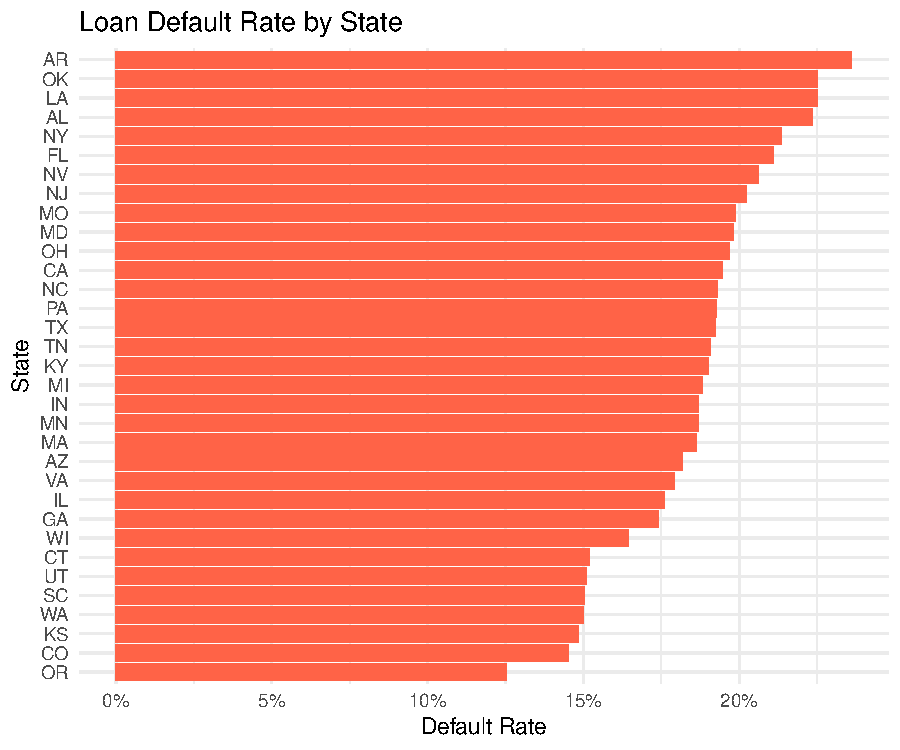
\includegraphics{22921893Question3_files/figure-latex/unnamed-chunk-6-1} 

}

\caption{Default rate for American states.}\label{fig:unnamed-chunk-6}
\end{figure}

\begin{figure}[H]

{\centering 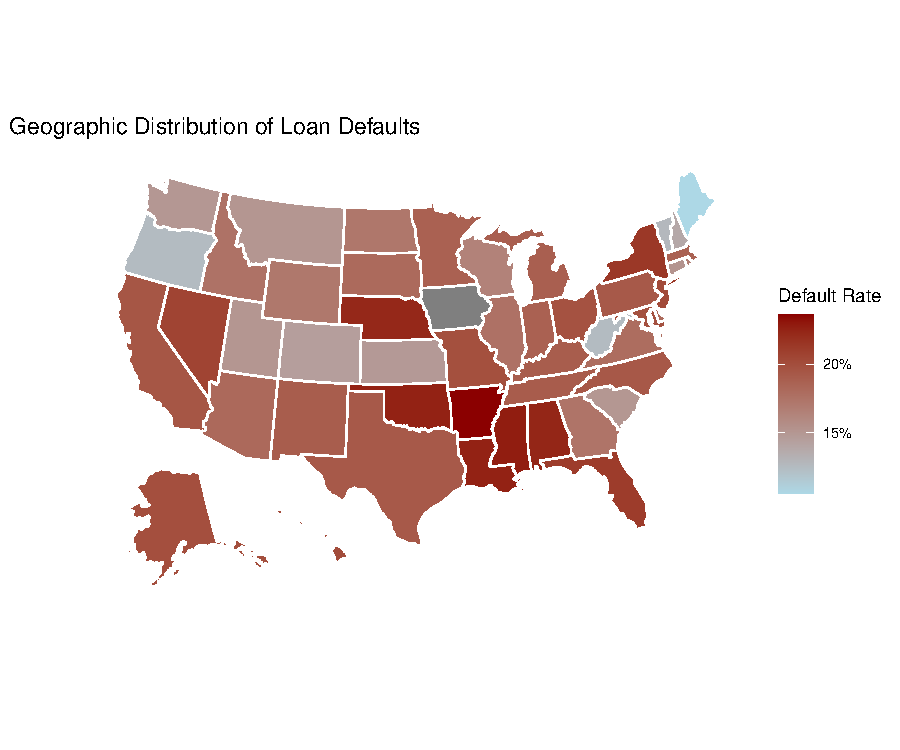
\includegraphics{22921893Question3_files/figure-latex/unnamed-chunk-7-1} 

}

\caption{Default rate in the United States}\label{fig:unnamed-chunk-7}
\end{figure}

\section{What does grade predict?}\label{what-does-grade-predict}

The following table displays the relationship between average default
rates and credit grades. As expected, the default rate rises steadily
from Grade A to Grade G. This indicates the credit grading system tracks
default risk well. The previous section highlighted two states of
interest, Arkansas and Oregon, representing the top and bottom of the
load default rate spectrum, respectively. Therefore, I plot the average
default rate for each credit rate for both these states. I add Texas as
it fell in the midrange of the state loan default rate.

\begin{longtable}[]{@{}lrr@{}}
\caption{Default rate by credit grade}\tabularnewline
\toprule\noalign{}
grade & n & default\_rate \\
\midrule\noalign{}
\endfirsthead
\toprule\noalign{}
grade & n & default\_rate \\
\midrule\noalign{}
\endhead
\bottomrule\noalign{}
\endlastfoot
G & 523 & 56.2 \\
F & 2141 & 48.0 \\
E & 9862 & 39.7 \\
D & 35625 & 32.5 \\
C & 83204 & 24.0 \\
B & 101540 & 15.2 \\
A & 64552 & 6.7 \\
\end{longtable}

As expected, Arkansas generally has a higher default rate at each credit
rating level, followed by Texas and Oregon. This indicates that the
grade-default relationship is consistent in this three state sub-sample.
The only exception is Grade G, which makes up a small amount of the
observations, indicating that the prominence of Grade G in the plot may
be unreliable.

\begin{figure}[H]

{\centering 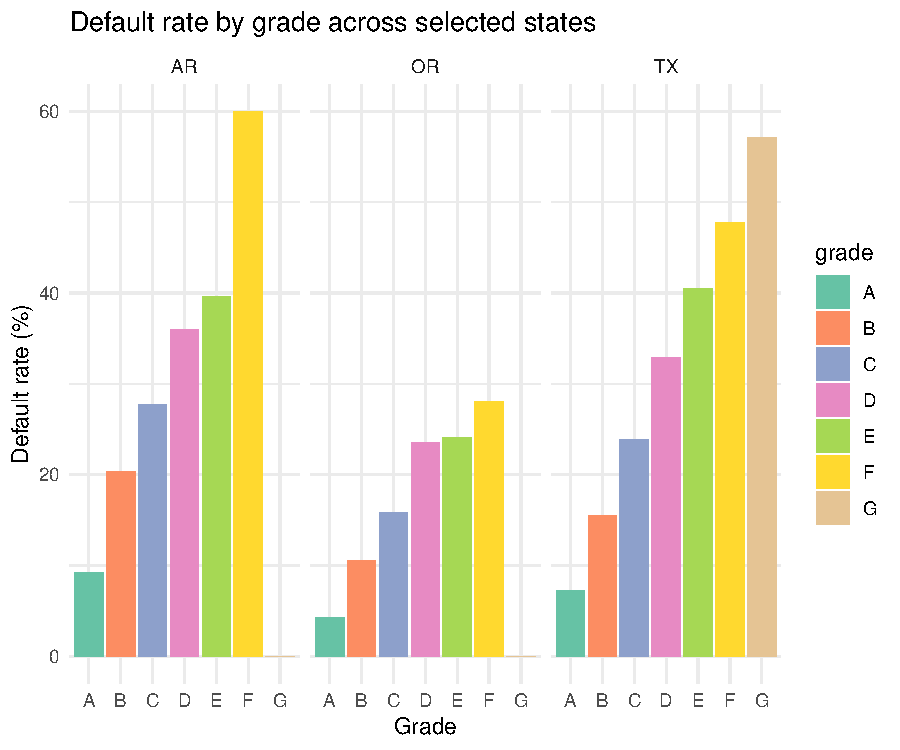
\includegraphics{22921893Question3_files/figure-latex/unnamed-chunk-9-1} 

}

\caption{Default rate by grade across Arkansas, Oregon, and Texas.}\label{fig:unnamed-chunk-9}
\end{figure}

\bibliography{Tex/ref}





\end{document}
